% !TEX root = ../00_tcc.tex

\begin{figure}[H]
	\centering
	\begin{subfigure}{\textwidth}
		\centering
		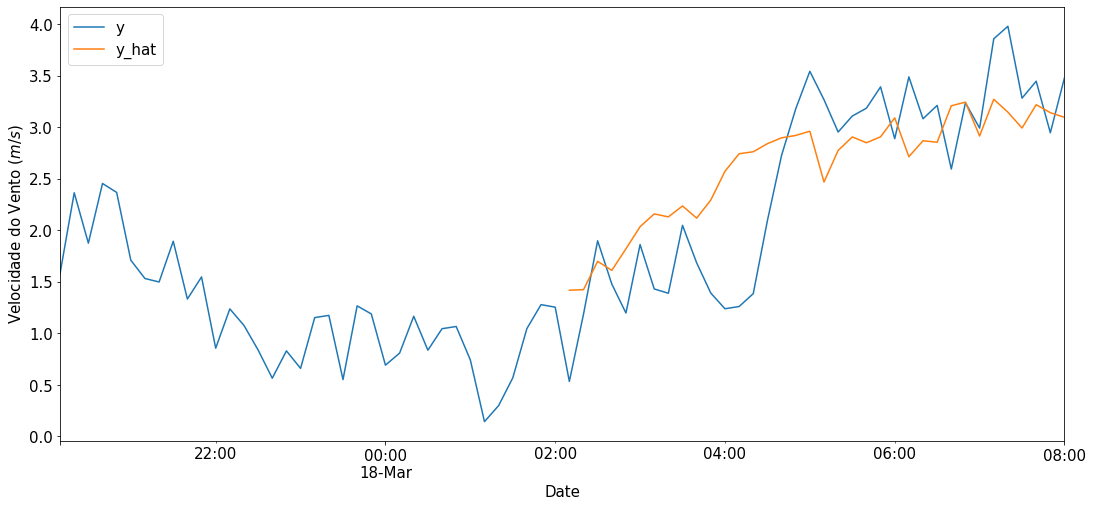
\includegraphics[width=0.8\textwidth]{../img/wind_comp.png}
		\caption{Previsão eólica}\label{fig:wind:comp}
	\end{subfigure}
	\\ \vspace{1cm}
	\begin{subfigure}{\textwidth}
		\centering
		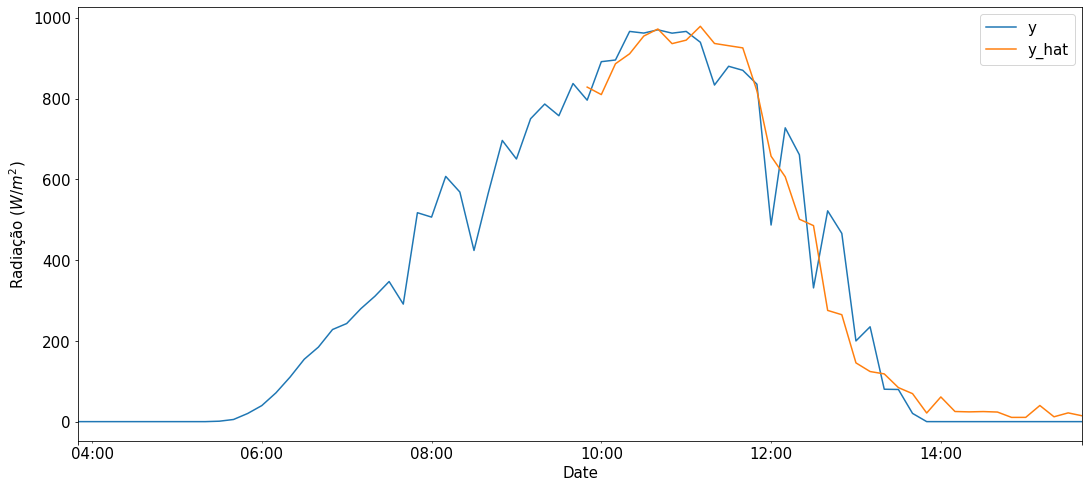
\includegraphics[width=0.8\textwidth]{../img/solar_comp.png}
		\caption{Previsão solar}\label{fig:solar:comp}
	\end{subfigure}
	\caption{Previsão final comparada aos dados reais}\label{fig:comp}
\end{figure}
